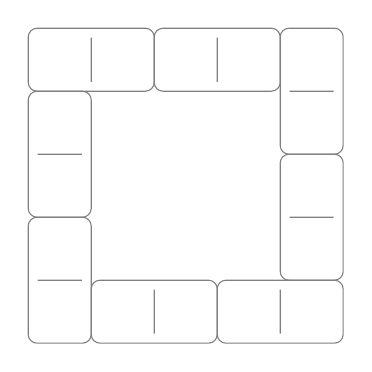
\begin{tikzpicture}[scale=.8]
\def\one{+(0.00,0.00) circle [radius=0.08]}
\def\two{+(-.25, .25) circle [radius=0.08]
	 +( .25,-.25) circle [radius=0.08]}
\def\thr{+(-.25, .25) circle [radius=0.08]
	 +(0.00,0.00) circle [radius=0.08]
	 +( .25,-.25) circle [radius=0.08]}
\def\fou{+(-.25,-.25) circle [radius=0.08]
	 +(-.25, .25) circle [radius=0.08]
	 +( .25,-.25) circle [radius=0.08]
	 +( .25, .25) circle [radius=0.08]}
\def\fiv{+(-.25,-.25) circle [radius=0.08]
	 +(-.25, .25) circle [radius=0.08]
	 +(0.00,0.00) circle [radius=0.08]
	 +( .25,-.25) circle [radius=0.08]
	 +( .25, .25) circle [radius=0.08]}
\def\six{+(-.25,-.25) circle [radius=0.08]
	 +(-.25, .25) circle [radius=0.08]
	 +(0.00,-.25) circle [radius=0.08]
	 +(0.00, .25) circle [radius=0.08]
	 +( .25,-.25) circle [radius=0.08]
	 +( .25, .25) circle [radius=0.08]}
\def\domino{
  [black,rounded corners=3.2pt]+(-1,-.5) rectangle +(1,.5)
  [gray,thin]+(0,.35) -- +(0,-.35)
}
\draw (-1.5, 2.0) \domino;
\draw ( 0.5, 2.0) \domino;
\begin{scope}[rotate=90]
  \draw (-1.5, 2.0) \domino;
  \draw ( 0.5, 2.0) \domino;
\end{scope}
\begin{scope}[rotate=180]
  \draw (-1.5, 2.0) \domino;
  \draw ( 0.5, 2.0) \domino;
\end{scope}
\begin{scope}[rotate=270]
  \draw (-1.5, 2.0) \domino;
  \draw ( 0.5, 2.0) \domino;
\end{scope}
\end{tikzpicture}
